\chapter{2D Blending and Deblending} \label{chap:theory}

This chapter recapitulates the idea behind blending and deblending. First the detail hiding operator notation is explained. This notation is used to describe the forward model of seismic data. By introducing the blending operator the forward model is extended to the blended case. Next, the deblending method presented in \citet{Mahdad-Deblending-Method} is discussed to illustrate some of the concepts used in this thesis.

\section{The Forward Model of Blending} \label{sec:Ch-Theory-Operator}
%The detail hiding operator notation was introduced by \citet{Berkhout1982}, and later on it was extended for blended data. 

\subsection{Conventional Seismic Data}
In the detail hiding operator notation \citep{Berkhout1982} the recorded signal is considered discrete in terms of time $t$\nomenclature{$t$}{Time}, receiver position $x_r$\nomenclature{$x_r$}{Receiver coordinates}, and source position $x_s$\nomenclature{$x_s$}{Source coordinates}. Thus, the measurements can be organized in a cube, $\mathbf{p}(t,x_r,x_s)$\nomenclature{$\mathbf{p}$}{3D data cube as a function of time, receiver coordinates, and source coordinates}, (see Figure \ref{fig:Ch-Theory-DataMatrix}). Each frequency slice of this new cube represents the data matrix, $\mathbf{P}$\nomenclature{$\mathbf{P}$}{(Monochromatic) data matrix as a function of receiver and source number}.

In the data matrix, $\mathbf{P}$, each column corresponds to a monochromatic common-shot gather (see Figure \ref{fig:Ch-Theory-DataMatrixMahdad}), each row to a monochromatic common-receiver gather, each diagonal to a monochromatic common-offset gather, and each anti-diagonal to a monochromatic common-midpoint gather. 

\begin{figure}
    \centering
	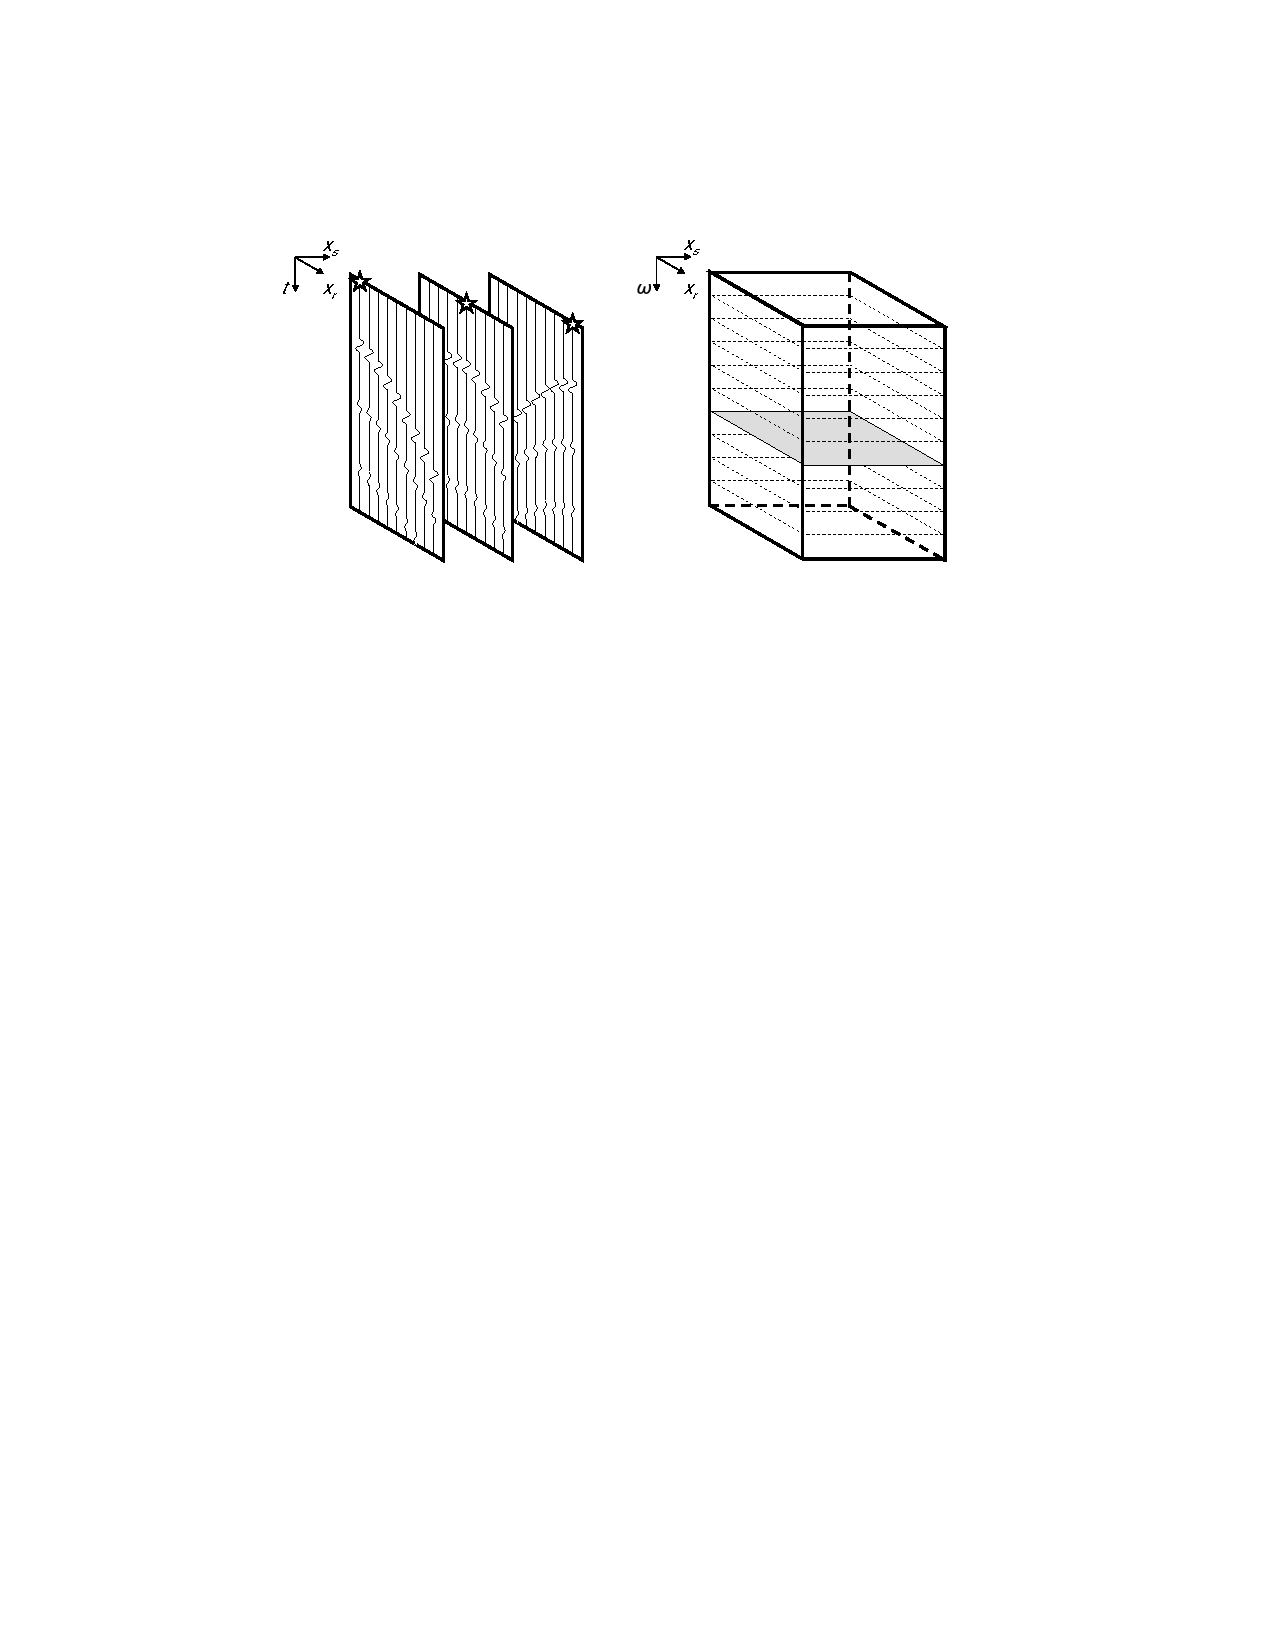
\includegraphics{Plots/P-Groenestijn_2010}
	\caption{Illustration of the data matrix, $\mathbf{P}$, by \citet{Groenestijn_2010}. \textit{Left:} The signal generated at the source position, $x_s$, is measured at receiver position, $x_r$, as a function of time, $t$. Thus, the discretized data is saved in a cube, $\mathbf{p}(t,x_r,x_s)$. \textit{Right:} The cube on the right equals the left cube after a Fourier transform with respect to time. Each frequency slice of the right cube represents the data matrix, $\mathbf{P}$.}
	\label{fig:Ch-Theory-DataMatrix}
\end{figure}


\begin{figure}
    \centering
	\includegraphics[width = 0.6\textwidth]{Plots/Mahdad-Data-Matrix-edited2}
	\caption{Illustration of the data matrix, $\mathbf{P}$, by \cite{Mahdad-Deblending-Method}. The dotted lines indicate directions of common gathers.}
	\label{fig:Ch-Theory-DataMatrixMahdad}
\end{figure}

According to the seismic forward model of \citet{Berkhout1982} the data matrix, $\mathbf{P}$, can be represented by a matrix multiplication of the source matrix, $\mathbf{S}$\nomenclature{$\mathbf{S}$}{(Monochromatic) source matrix as a function of source number}, the impulse response of the earth, $\mathbf{X}$\nomenclature{$\mathbf{X}$}{(Monochromatic) earth impulse response matrix as a function of receiver and source number}, and the receiver matrix, $\mathbf{D}$\nomenclature{$\mathbf{D}$}{(Monochromatic) receiver matrix as a function of receiver number}:

\begin{equation}
	\mathbf{P} = \mathbf{D \, X \, S}.
	\label{eq:Ch-Theory-DataRepresentation}
\end{equation}

In the source matrix, $\mathbf{S}$, both rows and columns represent shot positions (see Figure \ref{fig:Ch-Theory-BlendedSource}). Thus, $\mathbf{S}$ is a diagonal matrix. Each diagonal element $s_{ii}$\nomenclature{$s_{ii}$}{Diagonal element of the source matrix $\mathbf{S}$} captures one frequency component of the source signature injected in the earth at the position $x_s = x_i$\nomenclature{$x_i$}{Coordinates of the $i^{th}$ source}. By applying a Fourier transform to all frequency components of the element $s_{ii}$ the source signature as a function of time is obtained.

The impulse response of the earth, $\mathbf{X}$, describes how an impulse at the source location, $x_s$, is transformed in the earth into the signal at the receiver location, $x_r$.

The receiver matrix, $\mathbf{D}$, converts the seismic wavefield at the receiver location, $x_r$, to the recorded signal. This includes adding the receiver ghost.

In practice, one tries to retrieve the unknown earth response, $\mathbf{X}$, from the data, $\mathbf{P}$, by removing $\mathbf{S}$ (designature) and $\mathbf{D}$ (receiver deghosting).



\subsection{Blended Seismic Data}

\begin{figure}
	
	\centering
	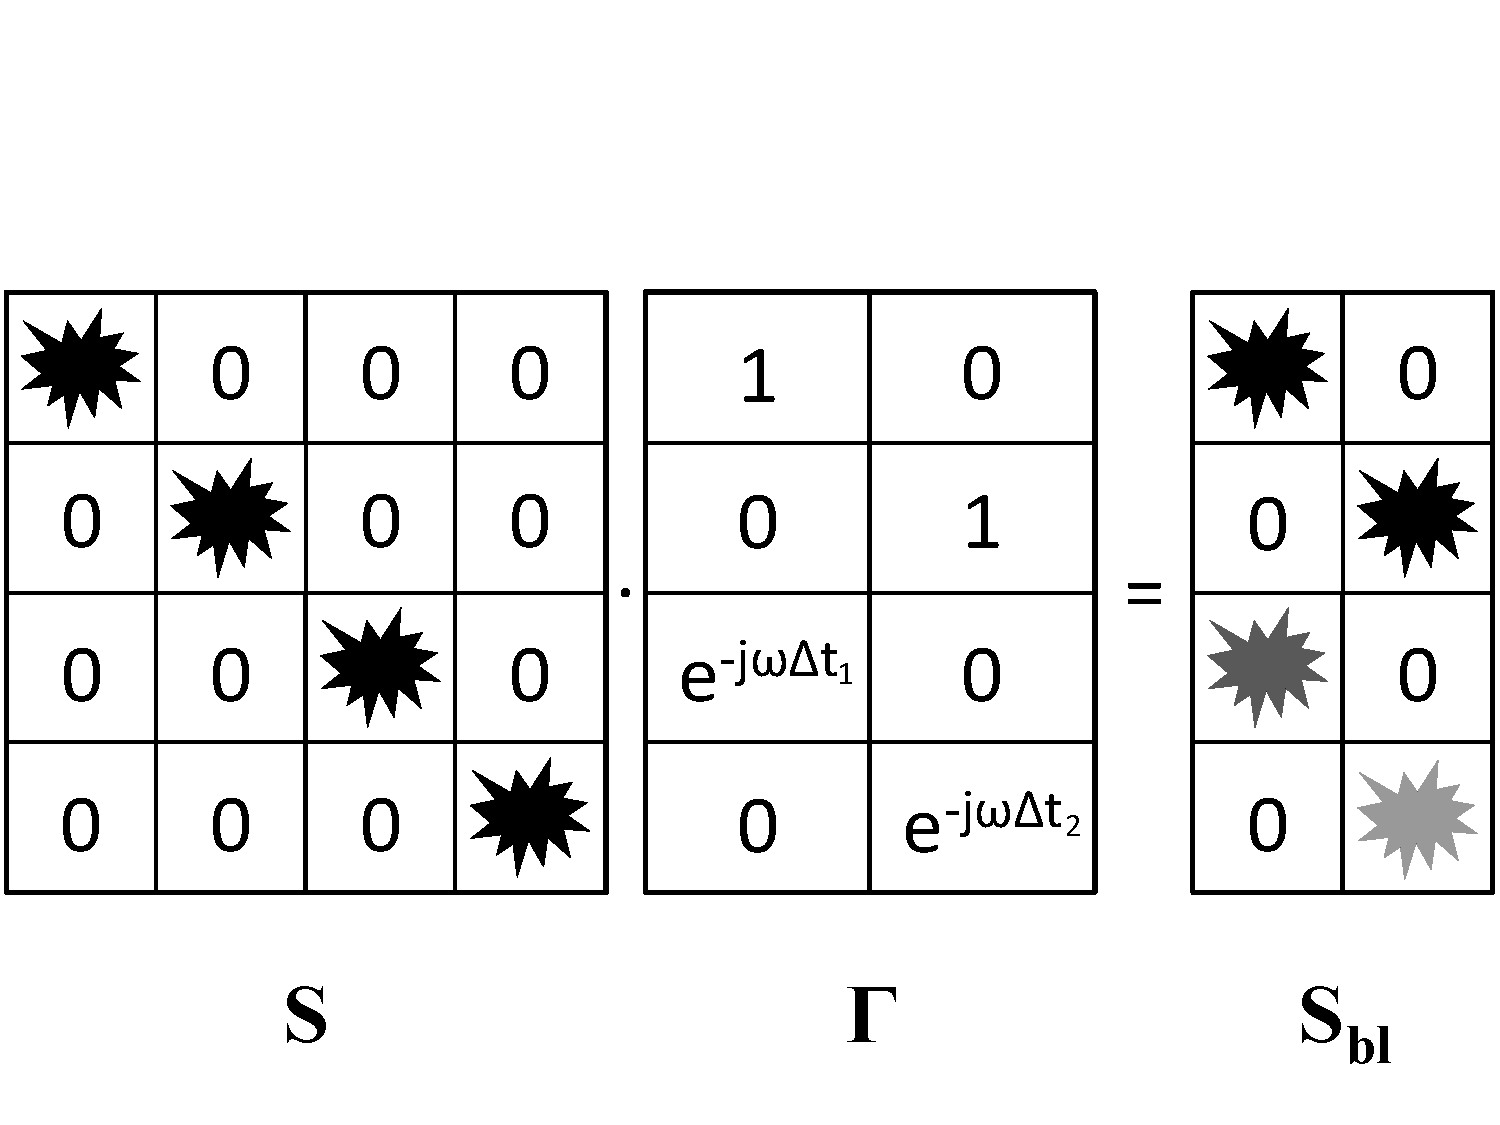
\includegraphics[width=0.6\textwidth]{Plots/Blended-Source-edit2}
	\caption{A conventional source matrix, $\mathbf{S}$, is transformed to a blended source matrix, $\mathbf{S}_{bl}$, by applying the blending matrix, $\mathbf{\Gamma}$. Each star represents one shot, and the gray scale of the stars represents the relative firing-time.}
	\label{fig:Ch-Theory-BlendedSource}
\end{figure}


\begin{comment}
\begin{figure}
	
	\centering
	\begin{subfigure}[t]{0.6\textwidth}	
	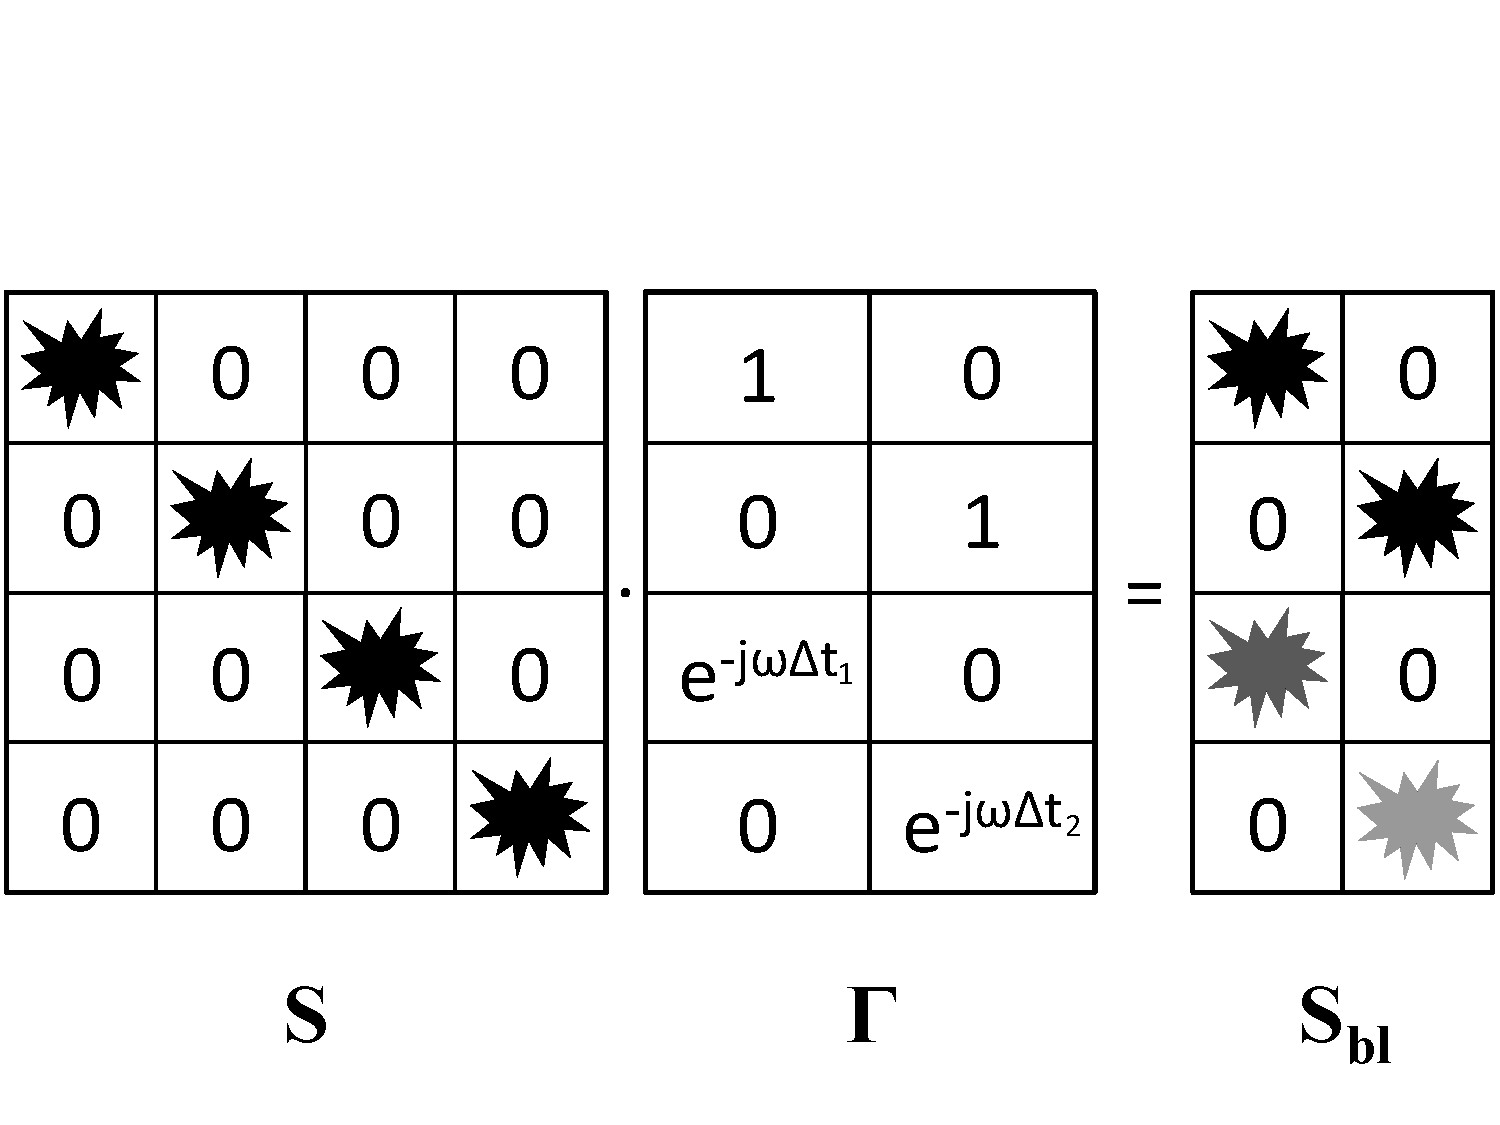
\includegraphics[width=\textwidth]{Plots/Blended-Source-edit2}
	\caption{}
	\label{fig:Ch-Theory-BlendedSource-Matrices}
	\end{subfigure}
	\par\bigskip
	\begin{subfigure}[t]{\textwidth}
	\centering
	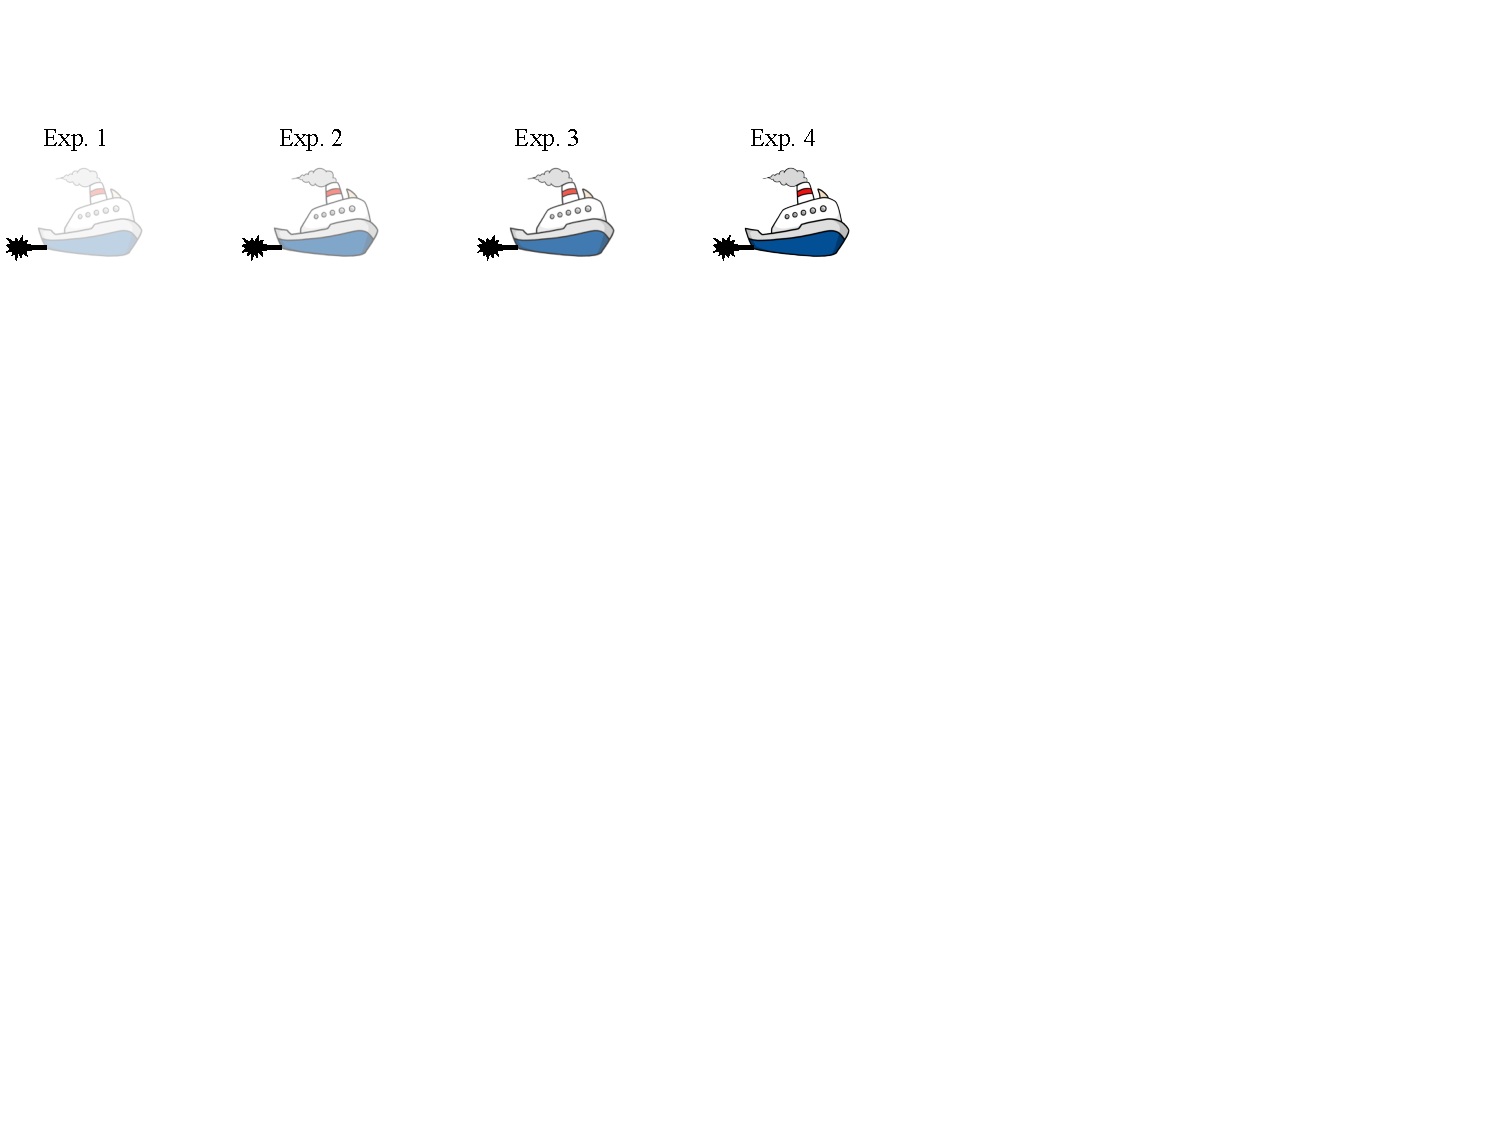
\includegraphics[width=0.5\textwidth]{Plots/Blended-Source-Conventional}
	\caption{}
	\label{fig:Ch-Theory-BlendedSource-Conventional}
	\end{subfigure}
	\par\bigskip
	\begin{subfigure}[t]{\textwidth}
	\centering
	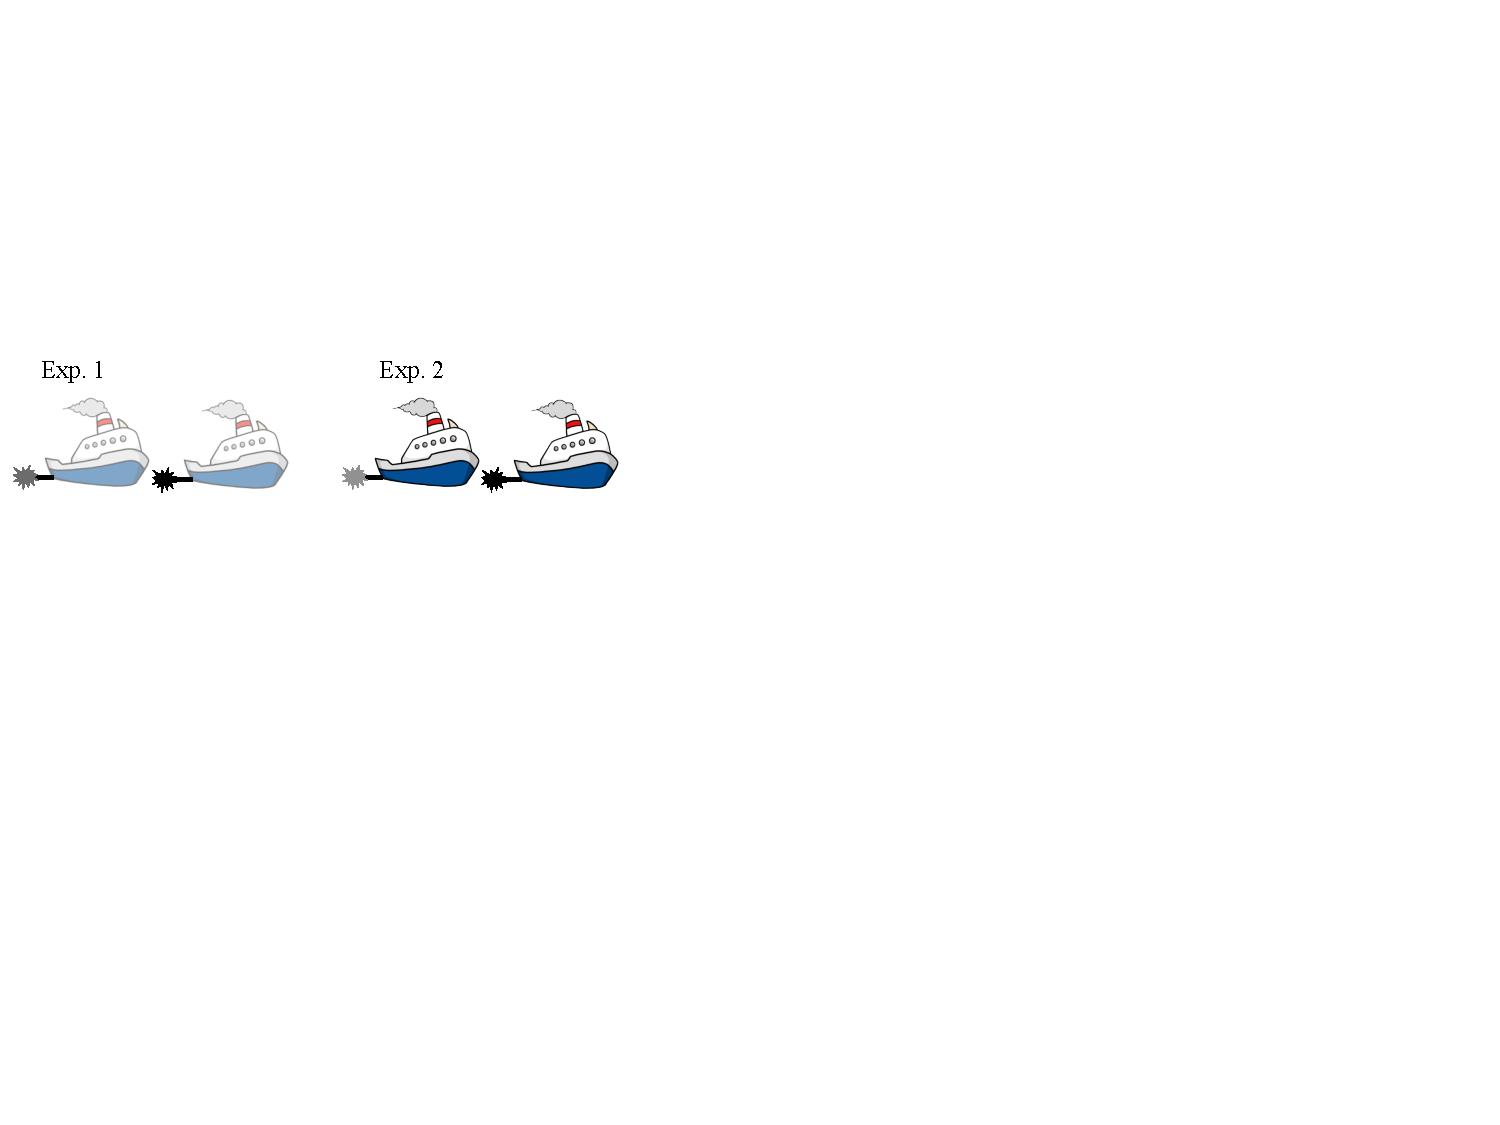
\includegraphics[width=0.36\textwidth]{Plots/Blended-Source-New}
	\caption{}
	\label{fig:Ch-Theory-BlendedSource-Blended}
	\end{subfigure}
    % RATIO of the boat images 294 : 410
	
	\caption{(a) A conventional source matrix, $\mathbf{S}$, is transformed to a blended source matrix, $\mathbf{S}_{bl}$, by applying the blending matrix, $\mathbf{\Gamma}$. Each star represents one shot, and the gray scale of the stars represents the relative firing time. (b) Illustration of conventional acquisition with one vessel. This acquisition set up is modeled by the source matrix $\mathbf{S}$. (c) Illustration of blended acquisition with two vessels. In this case the blended source matrix $\mathbf{S}_{bl}$ models the acquisition set up. The experiment number is indicated on top of each drawing.}
	\label{fig:Ch-Theory-BlendedSource}
	
\end{figure}
\end{comment}

In blended acquisition the recorded events belonging to different shots overlap, as shown in the shot gather in Figure \ref{fig:Ch-Theory-BlendedData}. 

\begin{figure}
	\centering
	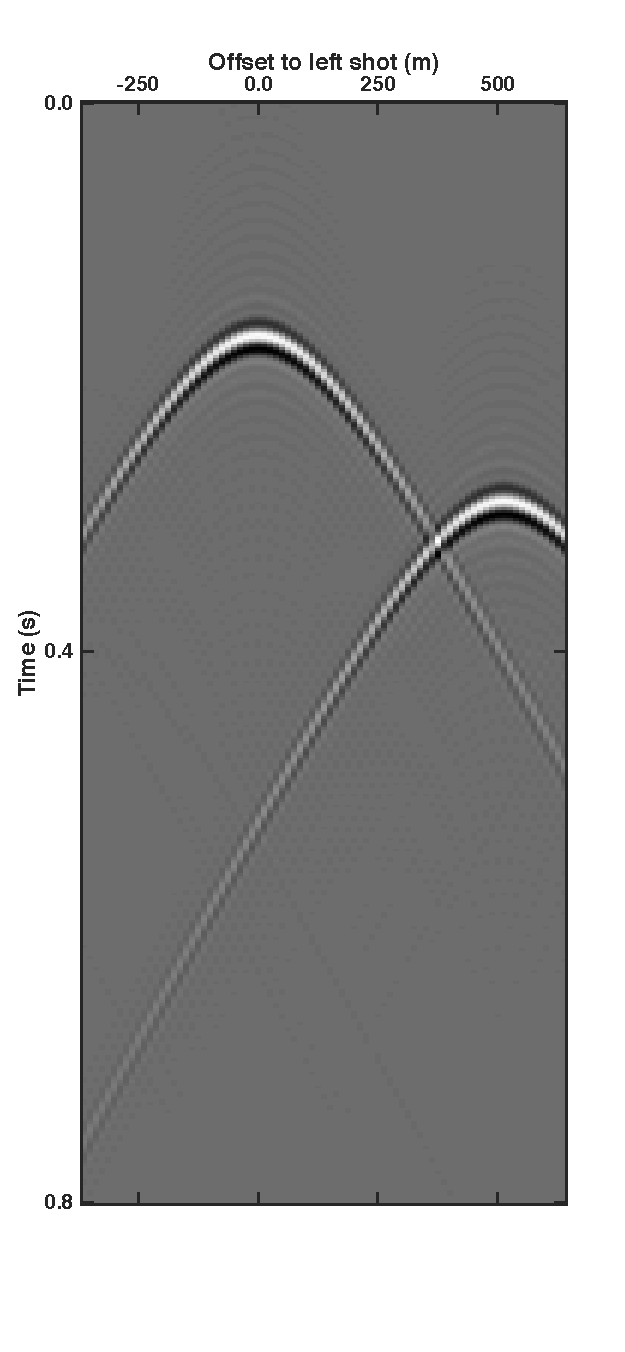
\includegraphics[width=0.25\textwidth]{Plots/Mahdad/30iter/BlendedCSG_sh1-edit_copy}
	\caption{Blended shot gather of two shots. The right shot is fired \SI{120}{\milli\second} after the left shot.}
	\label{fig:Ch-Theory-BlendedData}
\end{figure}

Blending can be captured in the forward model by introducing a blending matrix, $\mathbf{\Gamma}$\nomenclature{$\mathbf{\Gamma}$}{(Monochromatic) blending matrix as a function of source and experiment number}, which transforms the source matrix, $\mathbf{S}$, into a blended source matrix, $\mathbf{S}_{bl}$\nomenclature{$\mathbf{S}_{bl}$}{(Monochromatic) blended source matrix as a function of source and experiment number},

\begin{equation}
	\mathbf{S}_{bl} = \mathbf{S \, \Gamma}.
	\label{eq:Ch-Theory-BlendedSource}
\end{equation}

 Figure \ref{fig:Ch-Theory-BlendedSource} shows the structure of $\mathbf{\Gamma}$; each row of $\mathbf{\Gamma}$ represents one source, and each column of $\mathbf{\Gamma}$ represents one experiment with multiple shots. 
 
 The blending matrix captures the physics of a blended acquisition as follows: An element $\gamma_{ij}$\nomenclature{$\gamma_{ij}$}{Element of the blending matrix $\mathbf{\Gamma}$ corresponding to the $i^{th}$ source and the $j^{th}$ experiment} of the blending matrix includes a source $i$ and an experiment $j$. If the source $i$ is not fired in the $j^{th}$ experiment $\gamma_{ij}$ is zero. If it is fired, source $i$ has a relative amplitude $A_{ij}$\nomenclature{$A_{ij}$}{Amplitude of the element $\gamma_{ij}$ of the blending matrix $\mathbf{\Gamma}$} and a relative time delay $\Delta t_{ij}$\nomenclature{$\Delta t_{ij}$}{Time delay of the $i^{th}$ source in the $j^{th}$ experiment} with respect to the first source fired in the $j^{th}$ experiment;

\begin{equation}
	\gamma_{ij} =  A_{ij} \mathrm{e}^{-j \omega \Delta t_{ij}}.
	\label{eq:Ch-Theory-BlendingElement}
\end{equation}  
 
Thus, the blending matrix selects specific sources from the source matrix and superimposes them as visualized in Figure \ref{fig:Ch-Theory-BlendedSource}. From Figure \ref{fig:Ch-Theory-BlendedSource} it also becomes clear that both the blending matrix, $\mathbf{\Gamma}$, and the blended source matrix, $\mathbf{S}_{bl}$, have more rows than columns, i.e. there are more sources than experiments. Thus, the acquisition is done in less time.

In the case of source blending the receiver matrix, $\mathbf{D}$, is not influenced. Of course, the earth impulse response, $\mathbf{X}$, is independent of the acquisition design. Hence, the blended data can be written as;

\begin{equation}
	\mathbf{P}_{bl} = \mathbf{D} \, \mathbf{X} \, \mathbf{S}_{bl} = \mathbf{D} \, \mathbf{X} \, \mathbf{S} \, \mathbf{\Gamma} = \mathbf{P \, \Gamma}.
	\label{eq:Ch-Theory-BlendedData}
\end{equation}

Note that, the blended data matrix, $\mathbf{P}_{bl}$\nomenclature{$\mathbf{P}_{bl}$}{(Monochromatic) blended data matrix as a function of receiver and experiment number}, also has less columns, i.e. less experiments, than the unblended data matrix, $\mathbf{P}$.



\section{Deblending} \label{sec:MahdadMethod}

Before removing the receiver matrix, $\mathbf{D}$, and the source matrix, $\mathbf{S}$, one must remove  the blending matrix, $\mathbf{\Gamma}$, from the blended data, $\mathbf{P}_{bl}$. This process is called deblending.

The deblending method presented in this thesis builds on the method of \citet{Mahdad-Deblending-Method}. Therefore, this method is described in more detail.

The basic workflow of the Mahdad method is summarized in Figure \ref{fig:Ch-Theory-FlowChart} and will be explained step by step in the following subsections. 

\begin{figure}
	\centering
	\includegraphics[width=0.8\textwidth]{Plots/Mahdad-FlowChart-v6}
	\caption{Flowchart belonging to the deblending method of \citet{Mahdad-Deblending-Method}.}
	\label{fig:Ch-Theory-FlowChart}
\end{figure}

\subsection{Pseudo-Deblending}

Unfortunately, the inverse problem of equation \ref{eq:Ch-Theory-BlendedData} is underdetermined, which means that there is not a unique solution for the unblended data, $\mathbf{P}$. Thus, additional constraints are required to deblend the data, which are; (1) sparsity of the signal in the $x$-$t$-domain and (2) coherency of the signal in the $f$-$k$ domain. 

The first estimate of the unblended data matrix, $\mathbf{P}$, is obtained by pseudo-deblending;

\begin{equation}
	\mathbf{P}_{ps} = \mathbf{P}_{bl} \, \mathbf{\Gamma}^H,
	\label{eq:Ch-Theory-PseudoDeblended}
\end{equation}

where $\mathbf{\Gamma}^H$\nomenclature{$\mathbf{\Gamma}^{H}$}{(Monochromatic) conjugate transpose of the blending matrix $\mathbf{\Gamma}$ as a function of experiment and source number} is the conjugate transpose of the blending matrix, $\mathbf{\Gamma}$. Pseudo-deblending copies the blended data to the locations of all shots present in the blended shot and shifts them  upward in time to compensate for the time delay. For example, Figure \ref{fig:Ch-Theory-PseudoDeblendedCSG2} and \ref{fig:Ch-Theory-PseudoDeblendedCSG} shows the two pseudo-deblended shot gathers of the blended data in Figure \ref{fig:Ch-Theory-BlendedData}. Note that the pseudo-deblended data, $\mathbf{P}_{ps}$\nomenclature{$\mathbf{P}_{ps}$}{(Monochromatic) pseudo-deblended data matrix as a function of receiver and source number}, have the same size as $\mathbf{P}$.


\subsection{Common-Receiver Gather}

In Figure \ref{fig:Ch-Theory-PseudoDeblendedCSG2} and \ref{fig:Ch-Theory-PseudoDeblendedCSG} the interfering shot is coherent. By transforming the data to another domain, e.g. to the common-receiver domain, the interfering shot becomes incoherent \todo{definition of incoherency?} and is visible as spiky noise (see Figure \ref{fig:Ch-Theory-PseudoDeblendedCRG}). Therefore, the interfering shots can be attenuated with a noise filter in the common-receiver domain. 

%\todo[inline]{MOVE TO EXTENSION PART: Considering the 1/b factor, the interfering source creates blending noise and scales the amplitude of the shot of interest. So, is it correct to set blending noise and interfering source equal?}

\begin{figure}
	\centering
	\begin{subfigure}[t]{0.25\textwidth}
		\centering
		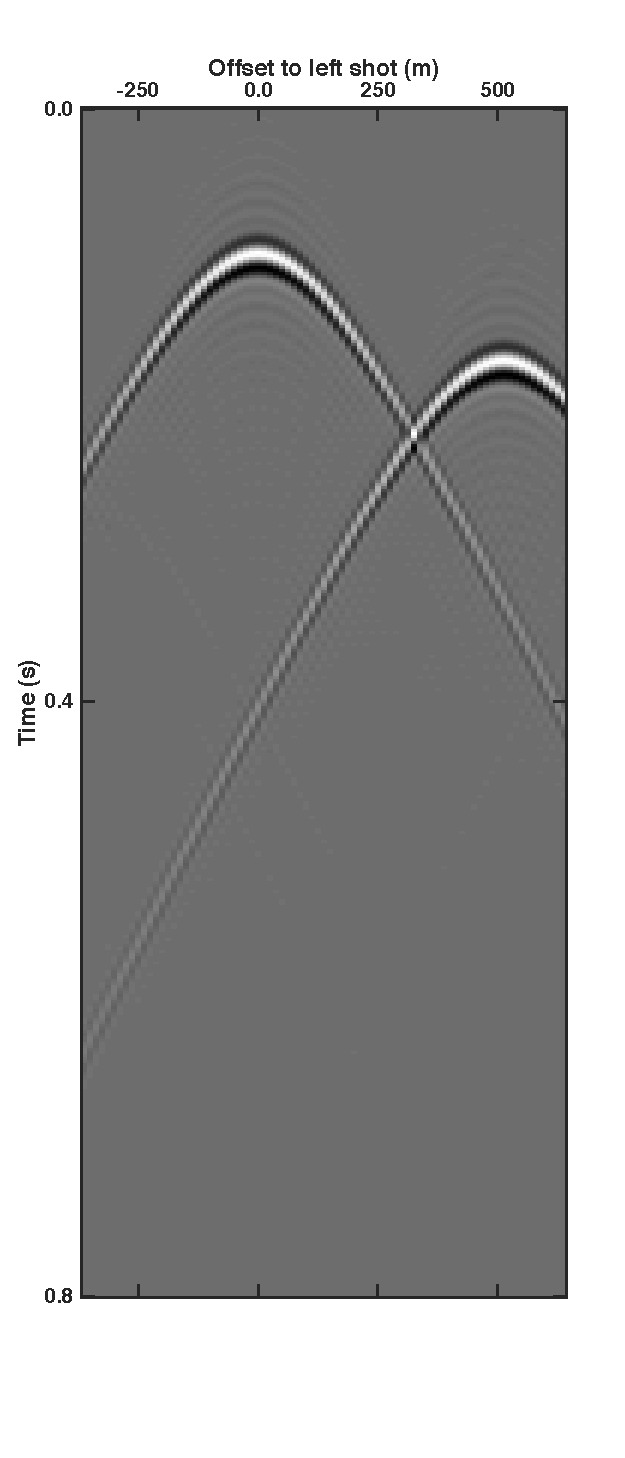
\includegraphics[width=0.925\textwidth]{Plots/Mahdad/30iter/Pseudo-DeblendedCSG_sh2}	
		\caption{Common-shot gather}
		\label{fig:Ch-Theory-PseudoDeblendedCSG2}
	\end{subfigure}
	%
	\centering
	\begin{subfigure}[t]{0.25\textwidth}
		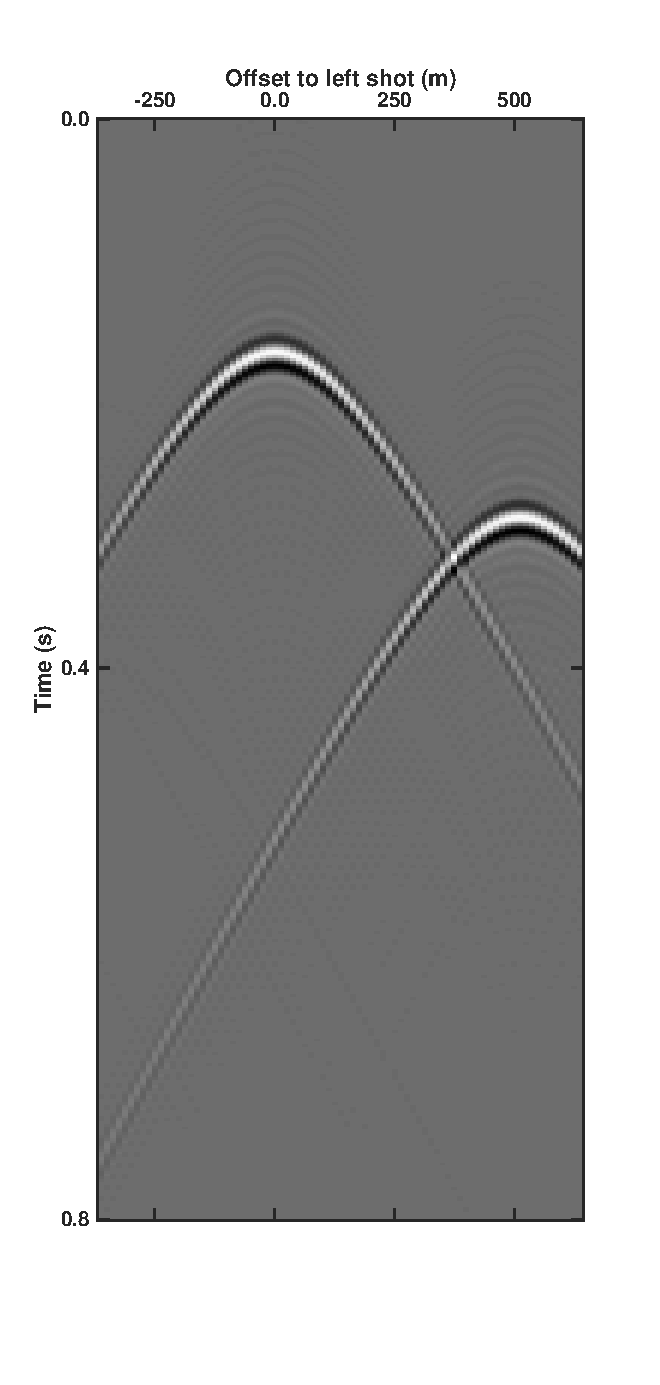
\includegraphics[width=\textwidth]{Plots/Mahdad/30iter/Pseudo-DeblendedCSG_sh1}	
		\caption{Common-shot gather}
		\label{fig:Ch-Theory-PseudoDeblendedCSG}
	\end{subfigure}
	%
	\centering
	\begin{subfigure}[t]{0.25\textwidth}
		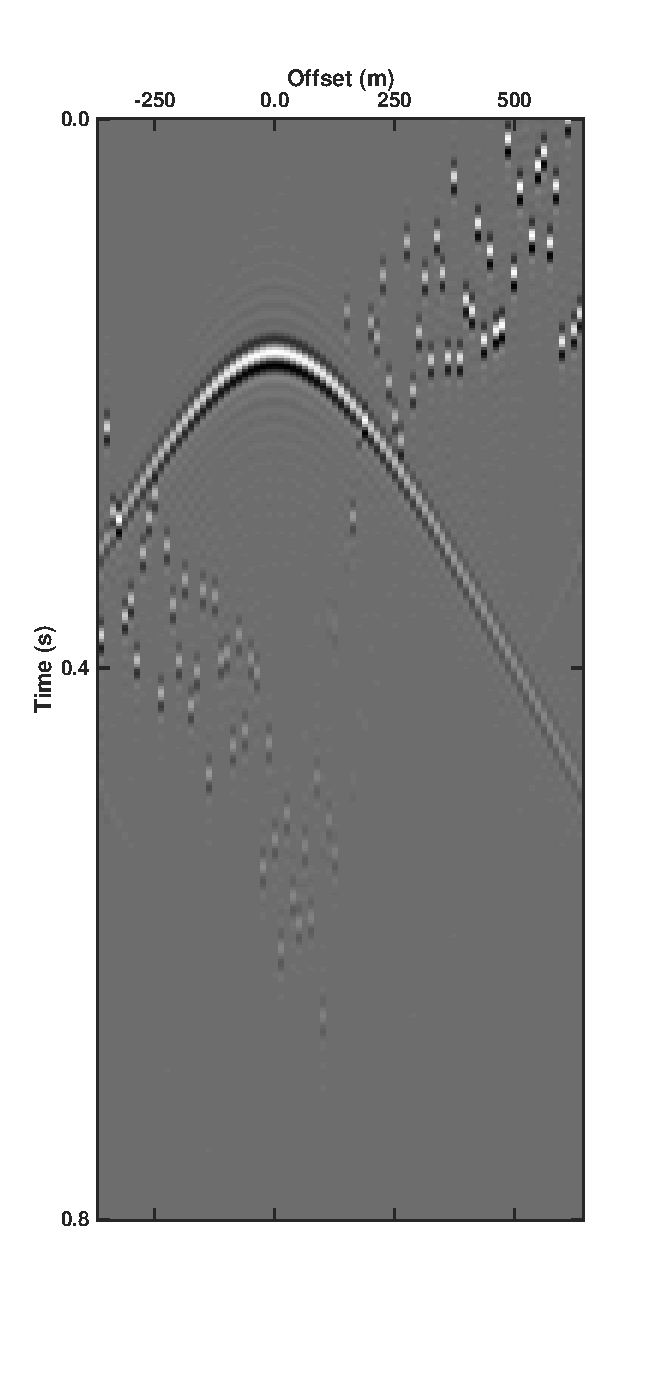
\includegraphics[width=\textwidth]{Plots/Mahdad/30iter/Pseudo-DeblendedCRG_rec30}	
		\caption{Common-receiver gather}
		\label{fig:Ch-Theory-PseudoDeblendedCRG}
	\end{subfigure}
	\caption{Pseudo-deblended data, $\mathbf{P}_{ps}$, sorted in common-shot gathers (a,b) and in a common-receiver gather (c). The pseudo-deblended data of the right shot (a) and the left shot (b,c) were shifted by different time delays. The overlapping sources map in the pseudo-deblended shot gathers as coherent events, while they map as incoherent spikes in the pseudo-deblended receiver gather.}
	\label{fig:Ch-Theory-PseudoDeblended}

\end{figure}


\subsection{Iterative Estimation of Blending Noise} \label{sec:IterBlenNoiseEst}

In an ideal case the noise generated by the interfering shots present in the pseudo-deblended data, the so-called blending noise, is calculated with the unblended data, \nomenclature{$\mathbf{N}$}{(Monochromatic) blending noise matrix as a function of receiver and source number}

\begin{equation}
	\mathbf{N} = \mathbf{P}_{bl} \, \mathbf{\Gamma}^H - \mathbf{P} = \mathbf{P}_{ps} - \mathbf{P}.
	\label{eq:Ch-Theory-Noise}
\end{equation}

Obviously, in practice the unblended data are unknown and are estimated by adding extra constraints. The loop shown in Figure \ref{fig:Ch-Theory-FlowChart} uses the pseudo-deblended data, $\mathbf{P}_{ps}$, as an initial estimation of the unblended data. Next, it applies the constraints to reduce the blending noise iteratively until the solution is obtained. 

In the following all the quantities which are estimated are indicated with a hat. The steps of the iterative blending noise estimation are illustrated in Figure \ref{fig:Ch-Theory-IterativeDeblending}.

\begin{figure}
	\centering
	\begin{subfigure}[t]{0.25\textwidth}
		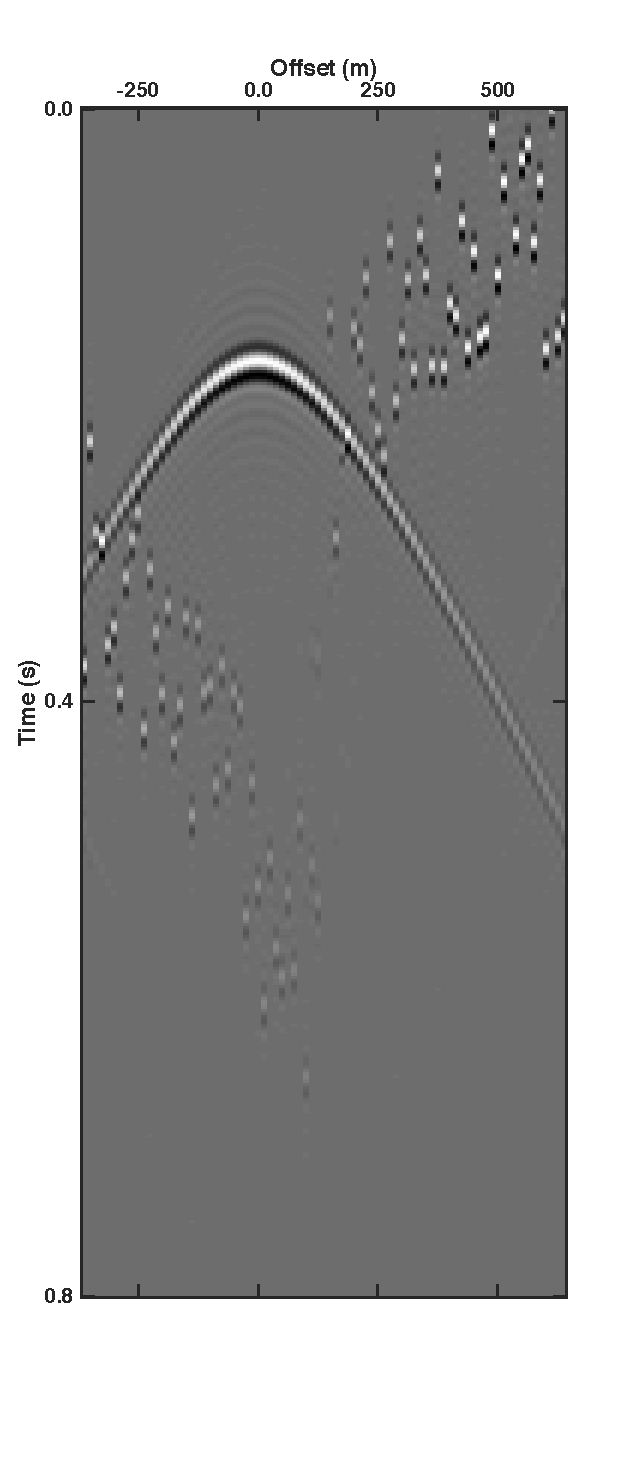
\includegraphics[width=\textwidth]{Plots/Mahdad/5iter/Pseudo-DeblendedCRG_rec30}	
		\caption{}
		\label{fig:Ch-Theory-PseudoDeblendedCRG5}
	\end{subfigure}
	%
	\centering
	\begin{subfigure}[t]{0.25\textwidth}
		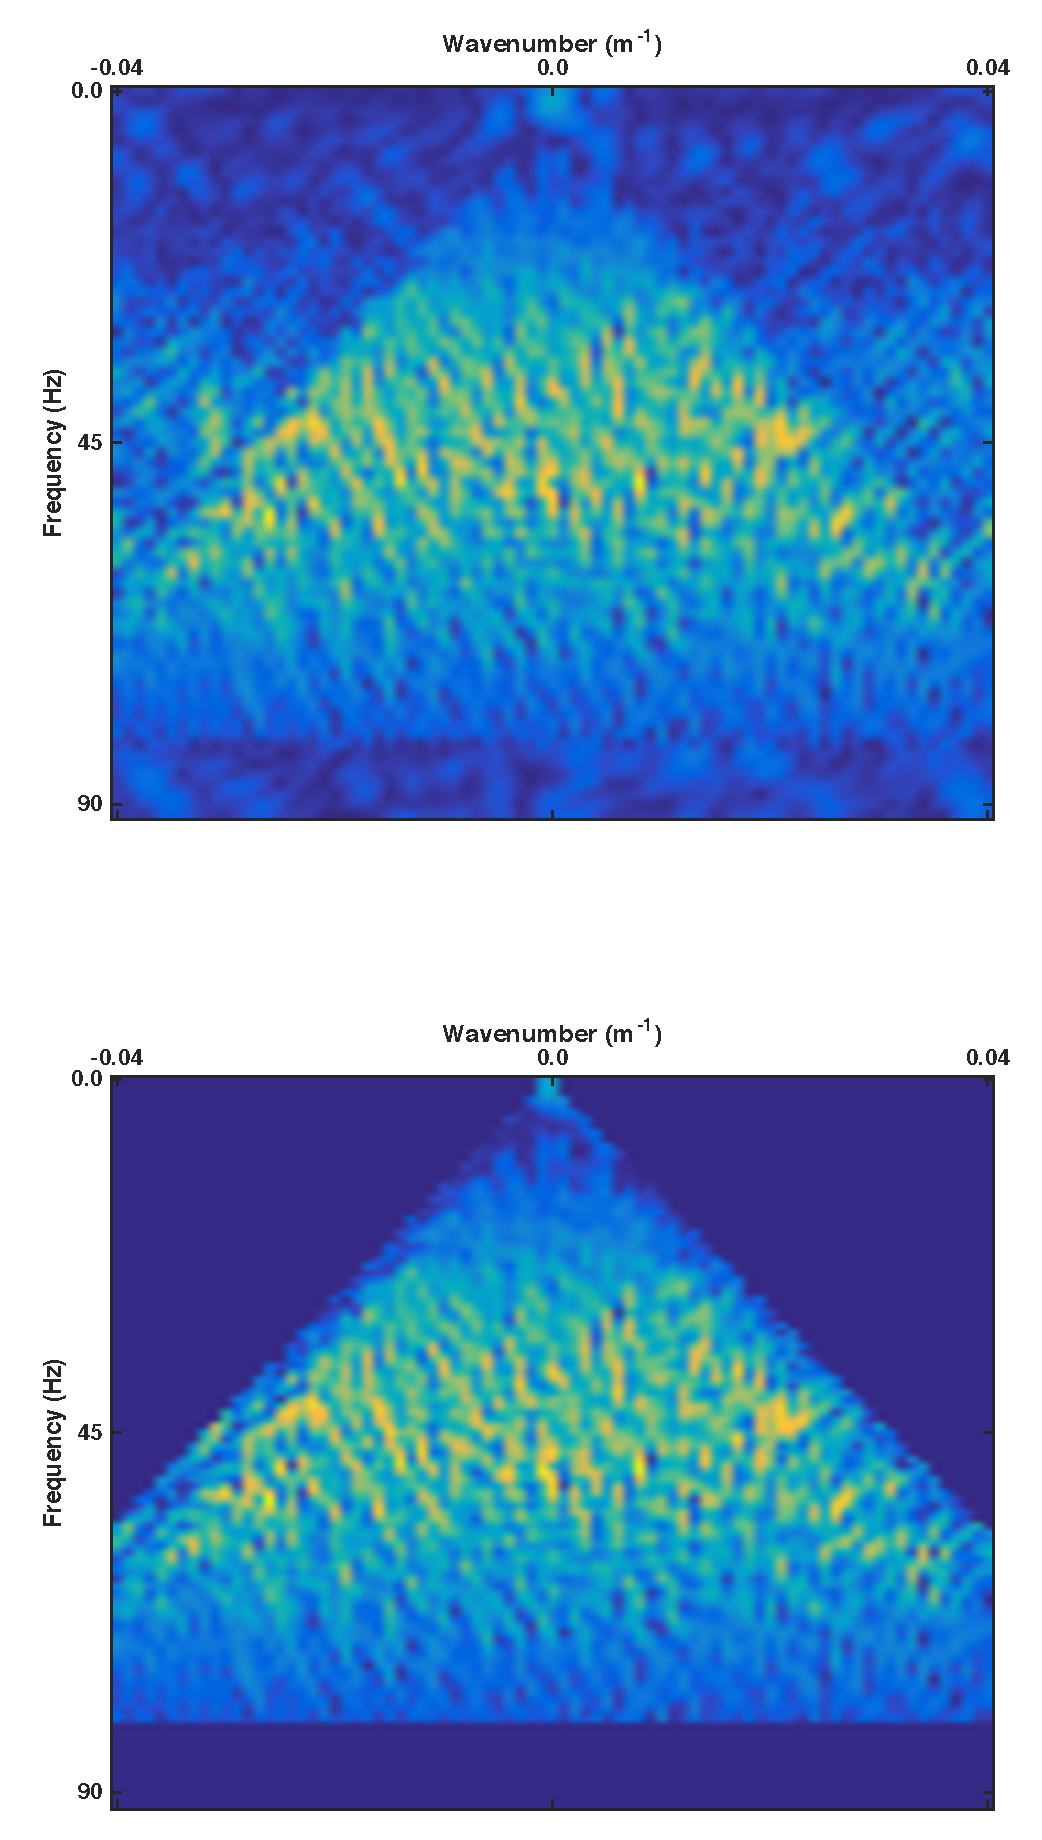
\includegraphics[width=\textwidth]{Plots/Mahdad/5iter/FK-Spectra}	
		\caption{}
		\label{fig:Ch-Theory-FKDeblended-NoFilter}
	\end{subfigure}
	%
	\begin{subfigure}[t]{0.25\textwidth}
		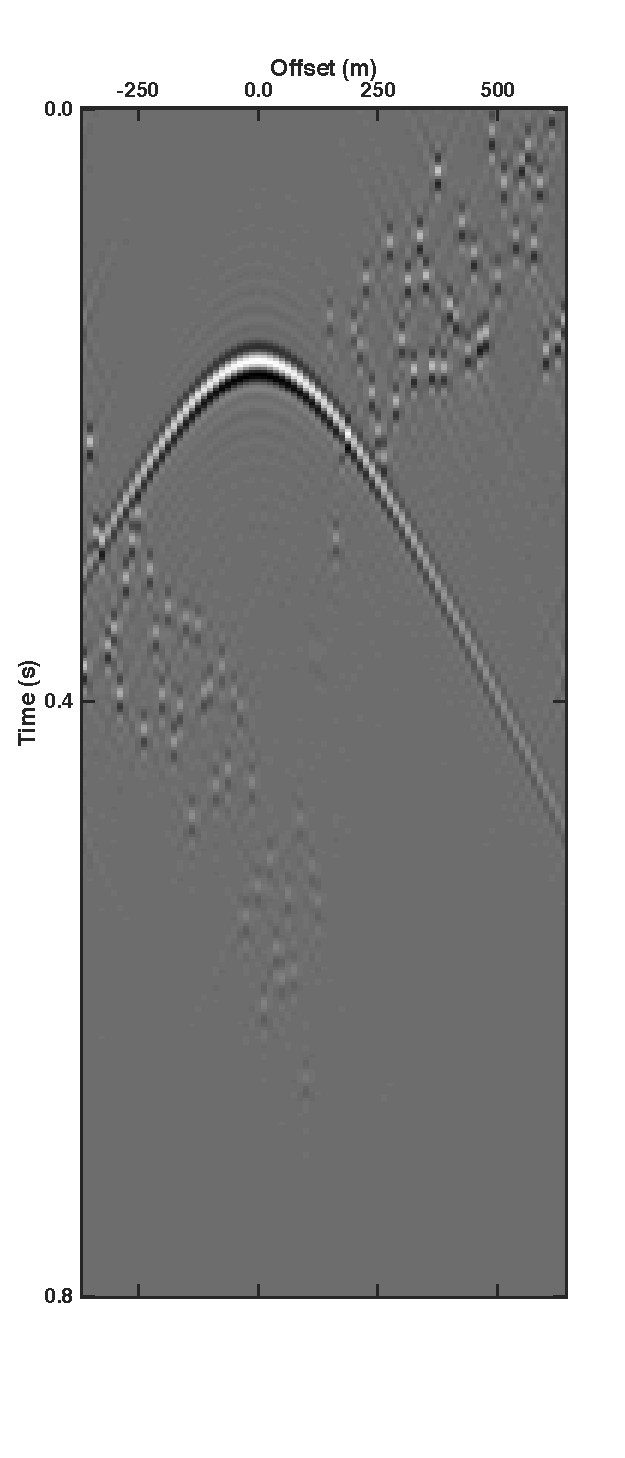
\includegraphics[width=\textwidth]{Plots/Mahdad/5iter/FkFilteredCRG_rec30}	
		\caption{}
		\label{fig:Ch-Theory-FKFiltered}
	\end{subfigure}
	%
	\begin{subfigure}[t]{0.25\textwidth}
		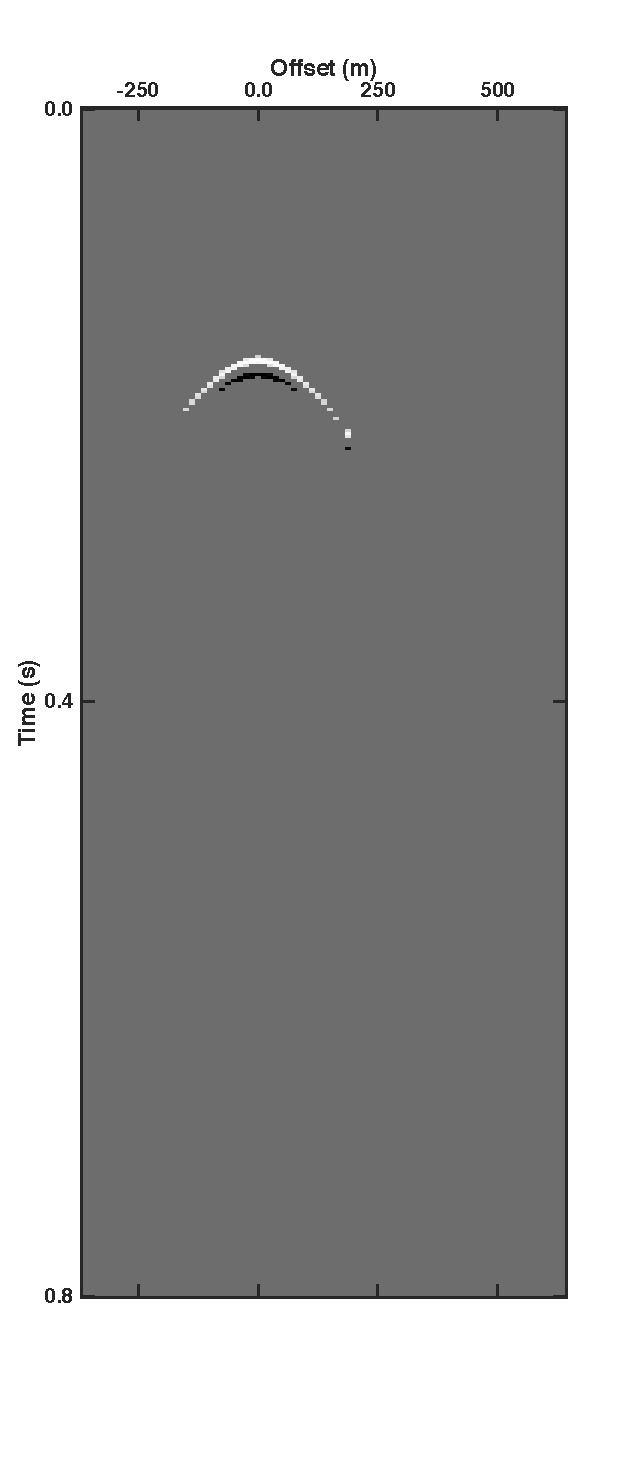
\includegraphics[width=\textwidth]{Plots/Mahdad/5iter/ThresholdCRG_rec30}	
		\caption{}
		\label{fig:Ch-Theory-Threshold}
	\end{subfigure}
	%
	\begin{subfigure}[t]{0.25\textwidth}
		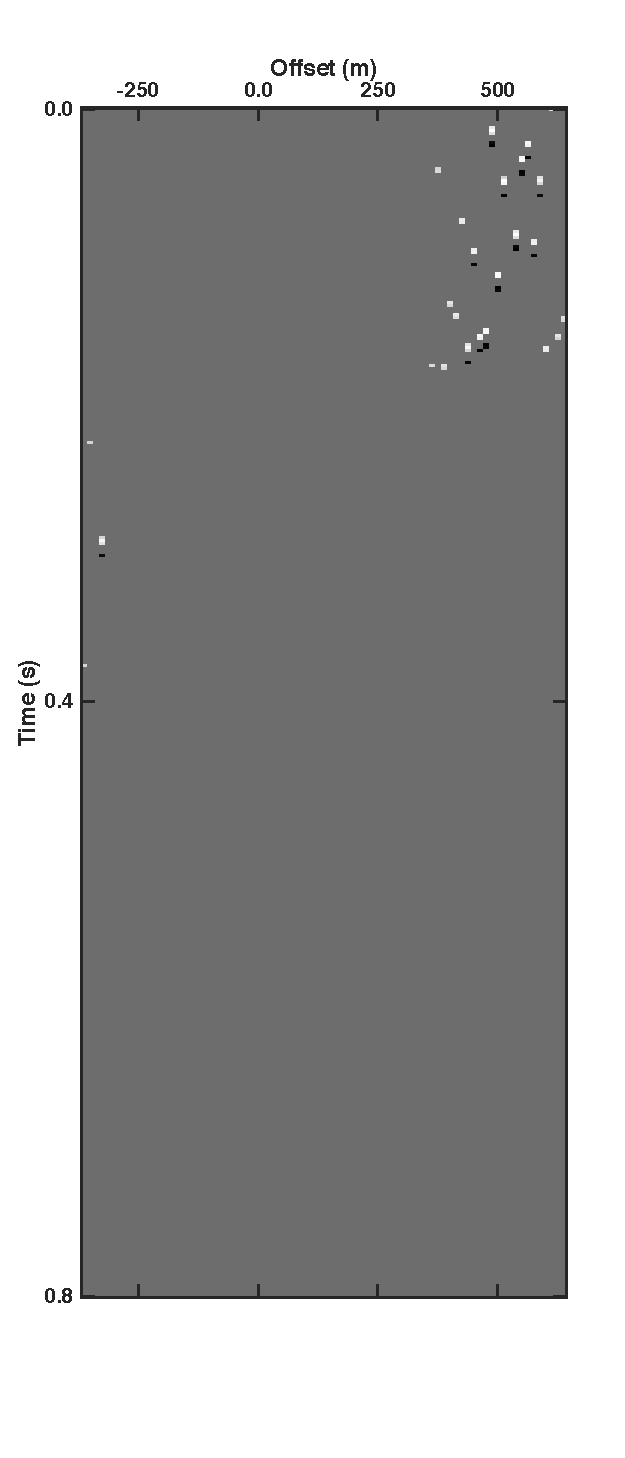
\includegraphics[width=\textwidth]{Plots/Mahdad/5iter/NoiseCRG_rec30}	
		\caption{}
		\label{fig:Ch-Theory-Noise}
	\end{subfigure}
	%
	\begin{subfigure}[t]{0.25\textwidth}
		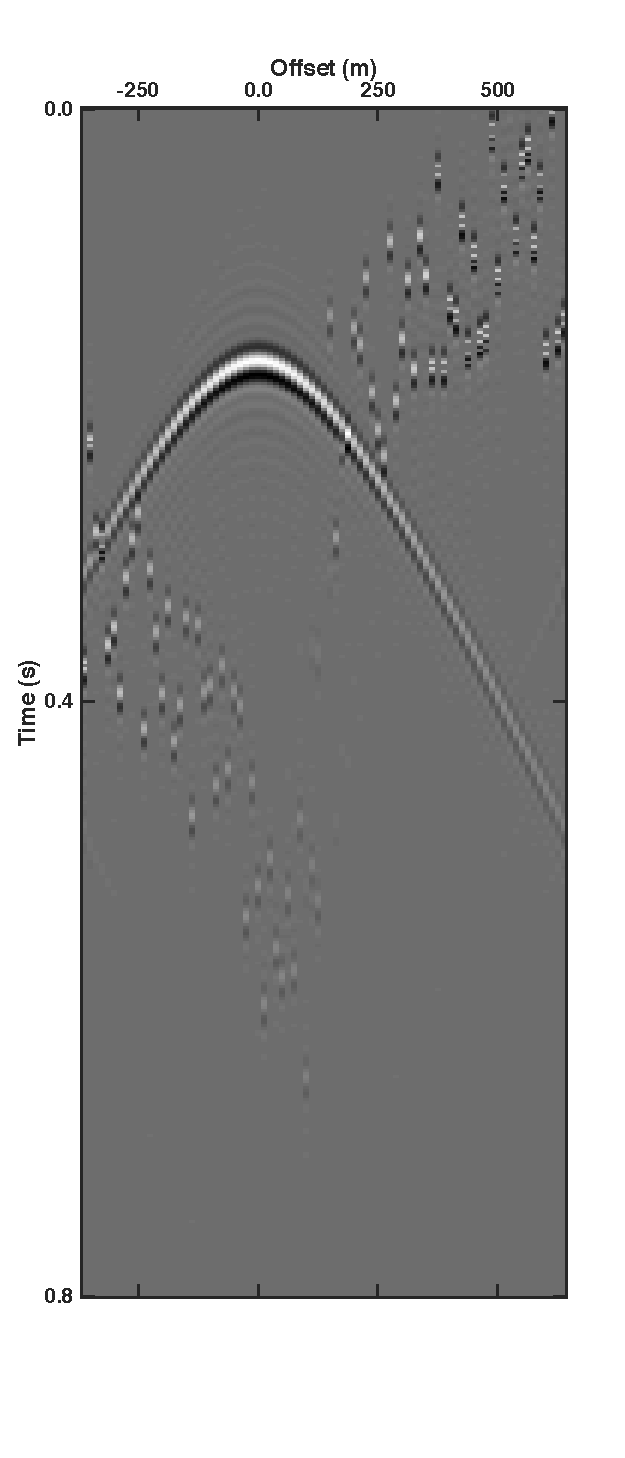
\includegraphics[width=\textwidth]{Plots/Mahdad/5iter/DeblendedCRG_rec30}	
		\caption{}
		\label{fig:Ch-Theory-Deblended}
	\end{subfigure}
	\caption{(a) Pseudo-deblended receiver gather. The subfigures (b)-(f) illustrate each step of the deblending algorithm. For better visibility examples from the $5^{th}$ iteration are chosen. (b) $f$-$k$ spectrum before (top) and after (bottom) $f$-$k$ filtering, (c) $f$-$k$ filtered common-receiver gather, (d) after thresholding, (e) estimated blending noise, (f) estimated data.}
	\label{fig:Ch-Theory-IterativeDeblending}
\end{figure}


\subsubsection*{f-k Filtering}

One of the constraints is coherency, i.e. by assuming the blending noise in Figure \ref{fig:Ch-Theory-PseudoDeblendedCRG5} is incoherent it can be removed. For this purpose the data are transformed from the space-time to the wavenumber-frequency domain where the spiky noise spreads over all wavenumber and frequency components (see Figure \ref{fig:Ch-Theory-FKDeblended-NoFilter}, top). 

%For a 2D $f$-$k$-spectrum the minimum (physical) velocity of the subsurface, $v_{min}$, determines the maximum wavenumber, $k_{max}$,  for a given frequency, $f$;

\nomenclature{$k$}{Wavenumber in a 2D case}
\nomenclature{$k_x$}{Crossline wavenumber in a 3D case}
\nomenclature{$k_y$}{Inline wavenumber in a 3D case}
The unblended data would map in the $f$-$k$ domain in a cone (see Figure \ref{fig:Ch-Theory-fk-Unblended-data}). The minimum wavefield velocity present in the subsurface, $v_{min}$\nomenclature{$v_{min}$}{Minimum wavefield velocity present in the subsurface}, determines the slope of the cone. This means that for a given frequency, $f$\nomenclature{$f$}{Frequency}, the maximum wavenumber inside the cone, $k_{max}$\nomenclature{$k_{max}$}{Maximum wavenumber for a given frequency $f$}, is defined as; 

\begin{equation}
	k_{max} = \frac{f}{v_{min}}.
	\label{eq_Ch-Theory-MaxWavenmber}
\end{equation} 

In the marine case the minimum velocity is usually the water velocity, $v_{w} = \SI{1500}{\metre\per\second}$\nomenclature{$v_w$}{Seismic velocity in water}.

\begin{figure}
	\centering
	\begin{subfigure}[t]{0.45\textwidth}
		\centering
		\includegraphics[width = \textwidth]{Plots/Mahdad/30iter/FK-UnblendedCSG_sh1_v2}
		\caption{$f$-$k$-spectrum of an unblended common-shot gather.}
		\label{fig:Ch-Theory-fk-Unblended-data}
	\end{subfigure}
	%
	\centering
	\begin{subfigure}[t]{0.45\textwidth}
		\centering
		\includegraphics[width = 0.957\textwidth]{Plots/Mahdad/30iter/FK-MaskCRG_rec30_v2}
		\caption{The $f$-$k$-mask is determined by the minimum signal velocity in the subsurface. The white area of the filter equals one, the black area equals zero. Thus, the filter removes data which are mapped outside of the white signal cone.}
		\label{fig:Ch-Theory-FK-Mask}
	\end{subfigure}
	
	\caption{}
	\label{fig:Ch-Theory-fk-unblended-data-mask}
\end{figure}

A 2D $f$-$k$ filter can be designed that removes all elements outside the cone (see Figure \ref{fig:Ch-Theory-FK-Mask}). The $f$-$k$ filter removes the part of the blending noise, which maps outside of the signal cone (see Figure \ref{fig:Ch-Theory-FKDeblended-NoFilter}). Thus, after transforming the data back to the space-time domain the amplitudes of the spiky noise are attenuated (see Figure \ref{fig:Ch-Theory-FKFiltered}). 

Note that $f$-$k$ filtering can only reduce spatially unaliased blending noise. In Figure \ref{fig:Ch-Theory-FK-Mask} the highest spatially unaliased frequency is defined by the point where the white cone intersects with the frequency axis, i.e. at \SI{60}{\hertz}. The spatially aliased blending noise will pass the $f$-$k$ filter and will be reduced afterwards by thresholding. 

The high cut frequency of the $f$-$k$ mask, $f_{cut} = \SI{80}{\hertz}$\nomenclature{$f_{cut}$}{High cut frequency of the $f$-$k$ mask}, is set according to the highest frequency components in the data. 

\subsubsection*{Thresholding}

The second constraint for the estimation of the unblended data is sparsity of the signal in the space-time domain.

After $f$-$k$ filtering the spiky noise is attenuated (see Figure \ref{fig:Ch-Theory-FKFiltered}). Consequently, the signal amplitudes are now stronger than the noise amplitudes. This allows to define a threshold in the $x$-$t$ domain, which is larger than the attenuated noise amplitudes and smaller than the highest signal amplitudes. Only amplitudes above the threshold are picked (see Figure \ref{fig:Ch-Theory-Threshold}). 

\subsubsection*{Interference Estimation}

The resulting thresholded data, \textbf{\={P}}\nomenclature{$\textbf{\={P}}$}{(Monochromatic) data matrix after thresholding as a function of receiver and source number}, is used to predict the blending noise;
\nomenclature{$\textbf{\^{N}}_{i}$}{(Monochromatic) blending noise prediction after $i$ iterations as a function of receiver and source number}
\nomenclature{$\mathbf{I}$}{Identity matrix}

\begin{equation}
	\textbf{\^{N}}_{i} = \textbf{\={P}} \, (\mathbf{\Gamma \, \Gamma^H} - \textbf{I}),
	\label{eq:Ch-Theory-NoiseEstimation}
\end{equation}

which is illustrated in Figure \ref{fig:Ch-Theory-Noise}.
 


\subsubsection*{Blending Noise Subtraction} 

The estimate of the unblended data matrix \textbf{\^{P}}$_{i}$ is updated by subtracting the estimated blending noise from the pseudo-deblended data,
\nomenclature{$\textbf{\^P}_{i}$}{(Monochromatic) data matrix prediction after $i$ iterations as a function of receiver and source number}

\begin{equation}
	\textbf{\^P}_{i+1} = \textbf{P}_{ps} - \textbf{\^{N}}_{i}, 
	\label{eq:Ch-Theory-DataUpdate1}
\end{equation}

which is shown in Figure \ref{fig:Ch-Theory-Deblended}.

This process is repeated iteratively till convergence is reached. In this context convergence can be defined as the point where the difference $\mid \textbf{\^P}_{i+1} - \textbf{\^{P}}_{i} \mid$ drops below a predefined limit. Alternatively, one can set a maximum number of iterations. 

Figure \ref{fig:Ch-Theory-EstimatedData} shows the estimate of the unblended data for increasing iterations. At each iteration the blending noise is attenuated further, such that the threshold can be lowered. Hence, the predicted blending noise increases and approaches the true blending noise. The two blended shots are successively  deblended.

Note that, $f$-$k$ filtering lowers the noise level by removing spatially unaliased blending noise. Next, the lowered noise level enables thresholding to reduce spatially aliased blending noise. Thus, the combination of $f$-$k$ filtering and thresholding is very powerful.


\begin{figure}
	\centering
	\begin{subfigure}[t]{0.25\textwidth}
		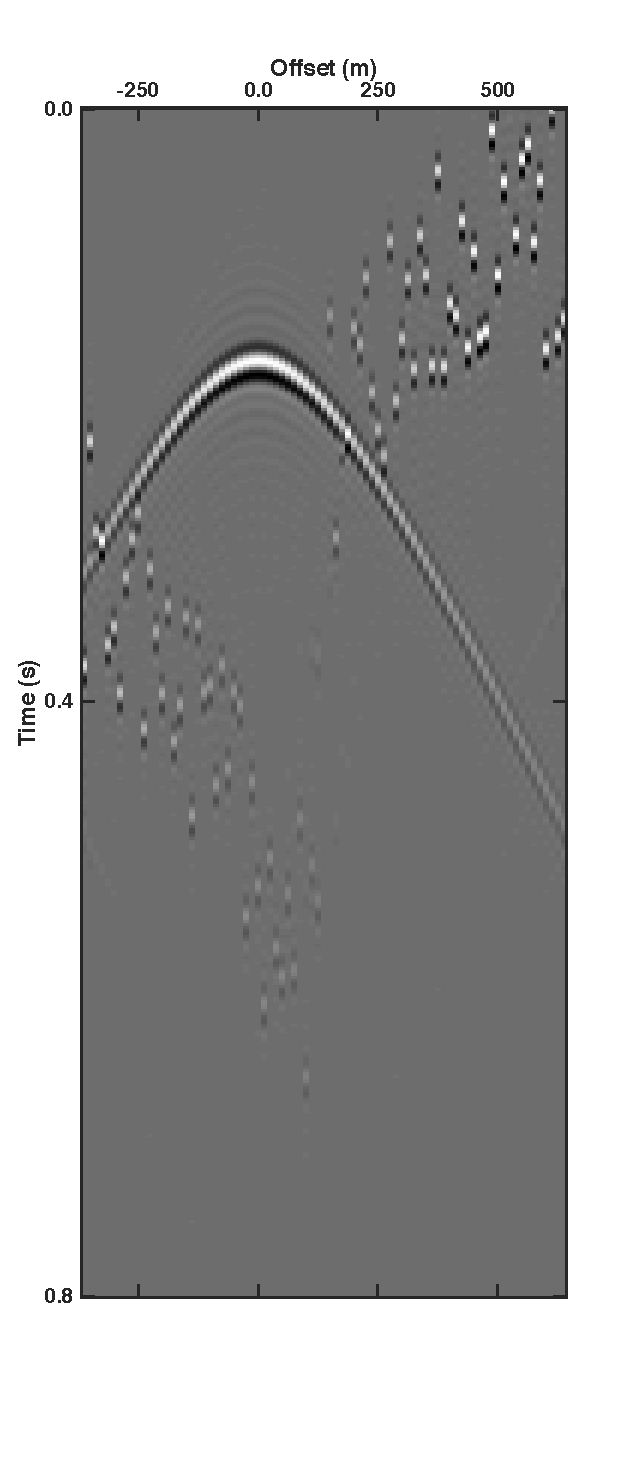
\includegraphics[width=\textwidth]{Plots/Mahdad/1iter/DeblendedCRG_rec30}	
		\caption{1 Iteration}
		\label{fig:Ch-Theory-DeblendedCRG1}
	\end{subfigure}
	%
	\centering
	\begin{subfigure}[t]{0.25\textwidth}
		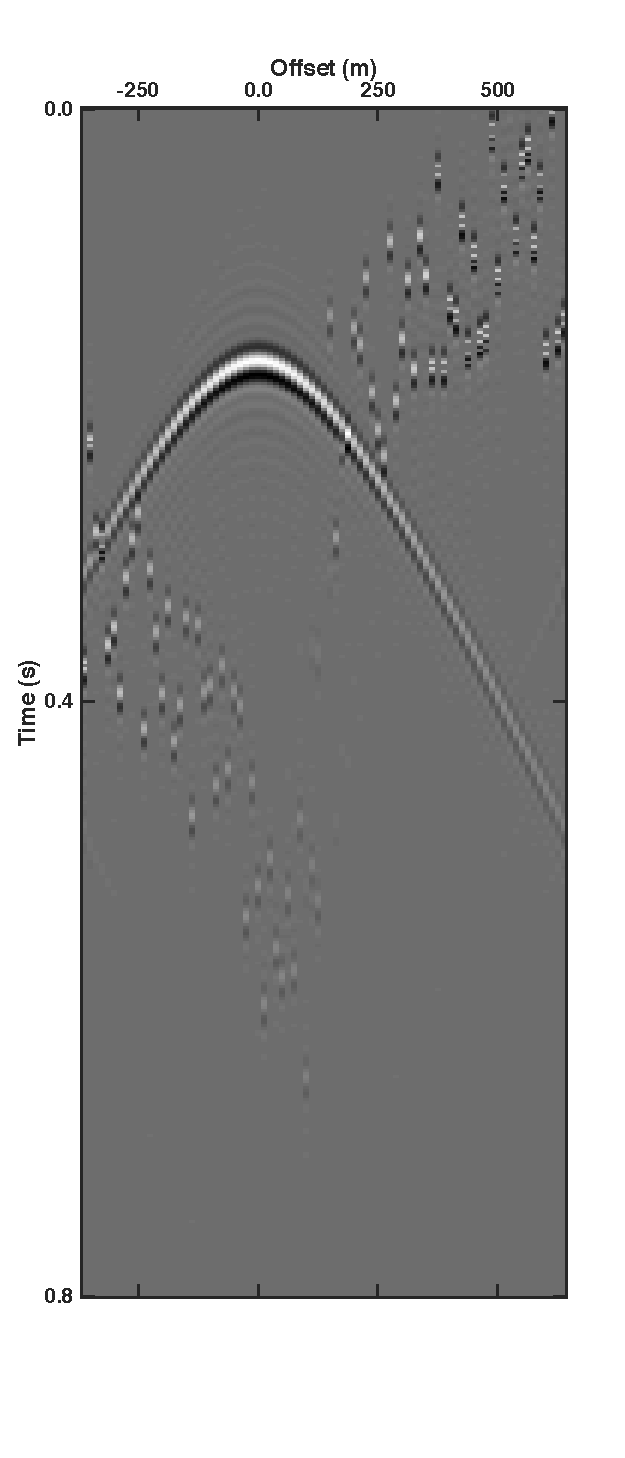
\includegraphics[width=\textwidth]{Plots/Mahdad/5iter/DeblendedCRG_rec30}	
		\caption{5 Iterations}
		\label{fig:Ch-Theory-DeblendedCRG5}
	\end{subfigure}
	%
	\begin{subfigure}[t]{0.25\textwidth}
		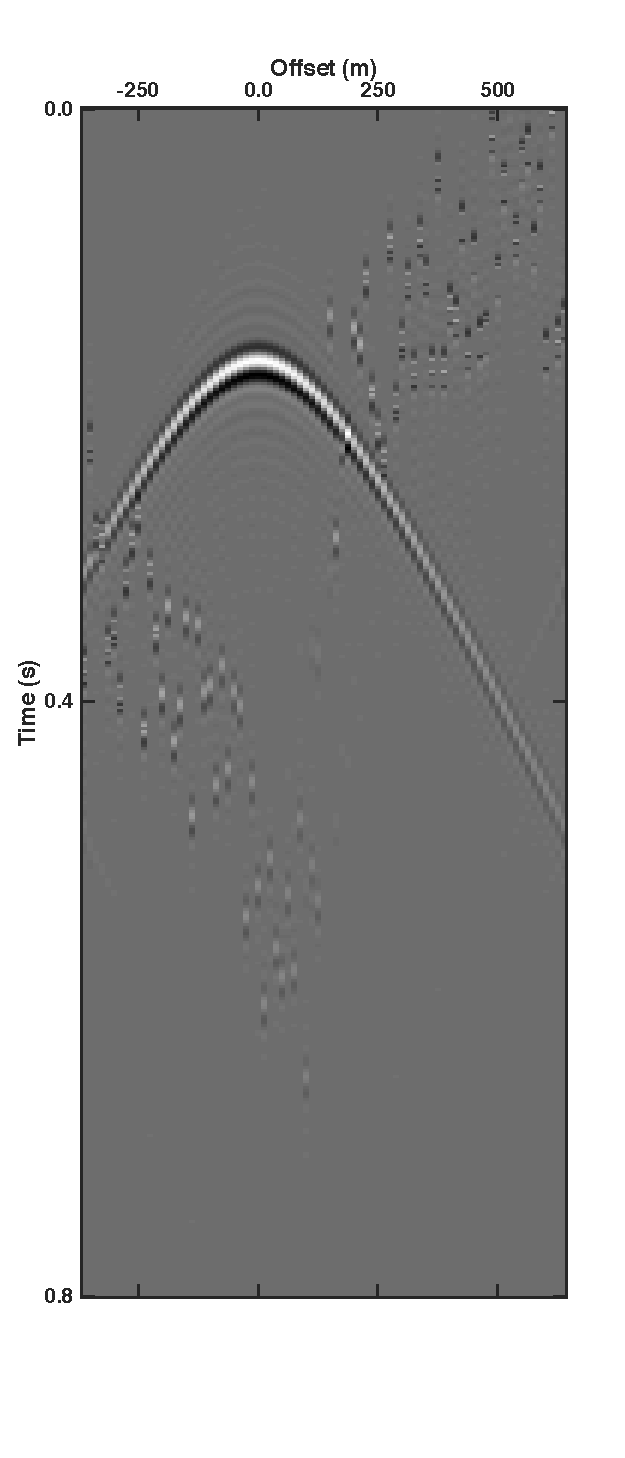
\includegraphics[width=\textwidth]{Plots/Mahdad/10iter/DeblendedCRG_rec30}	
		\caption{10 Iterations}
		\label{fig:Ch-Theory-DeblendedCRG10}
	\end{subfigure}
	%
	\begin{subfigure}[t]{0.25\textwidth}
		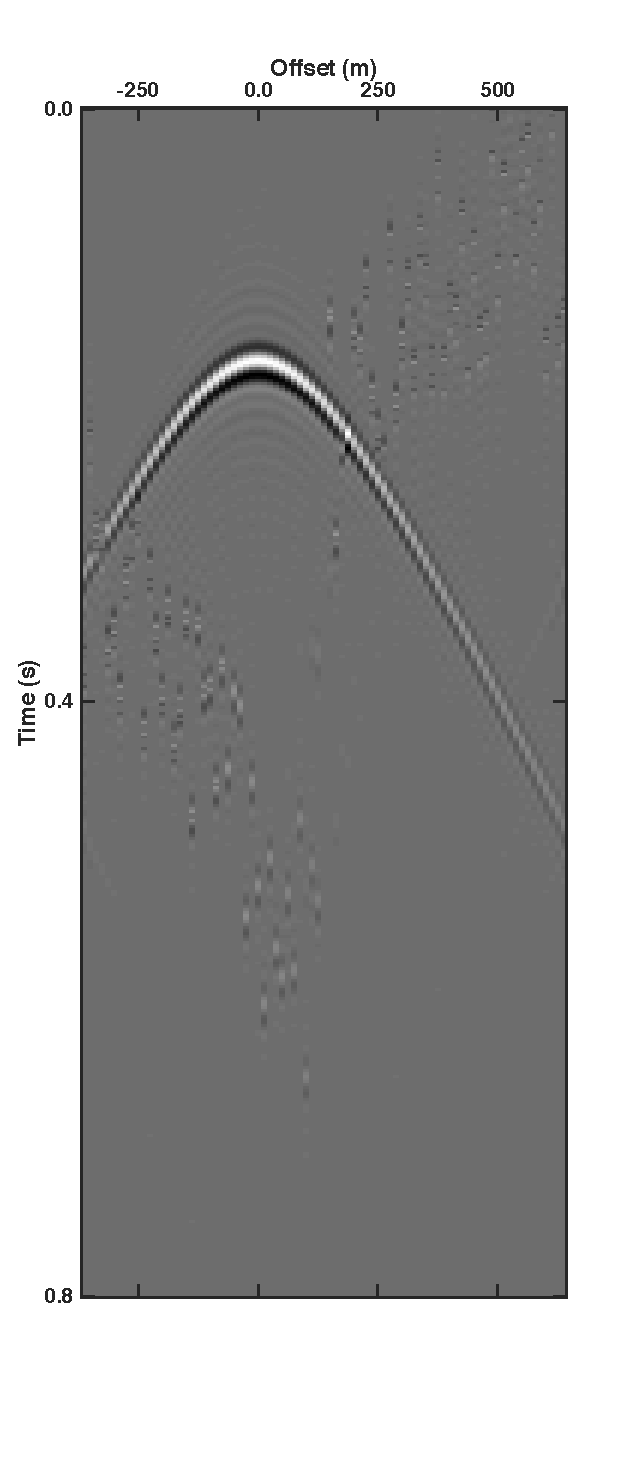
\includegraphics[width=\textwidth]{Plots/Mahdad/15iter/DeblendedCRG_rec30}	
		\caption{15 Iterations}
		\label{fig:Ch-Theory-DeblendedCRG15}
	\end{subfigure}
	%
	\begin{subfigure}[t]{0.25\textwidth}
		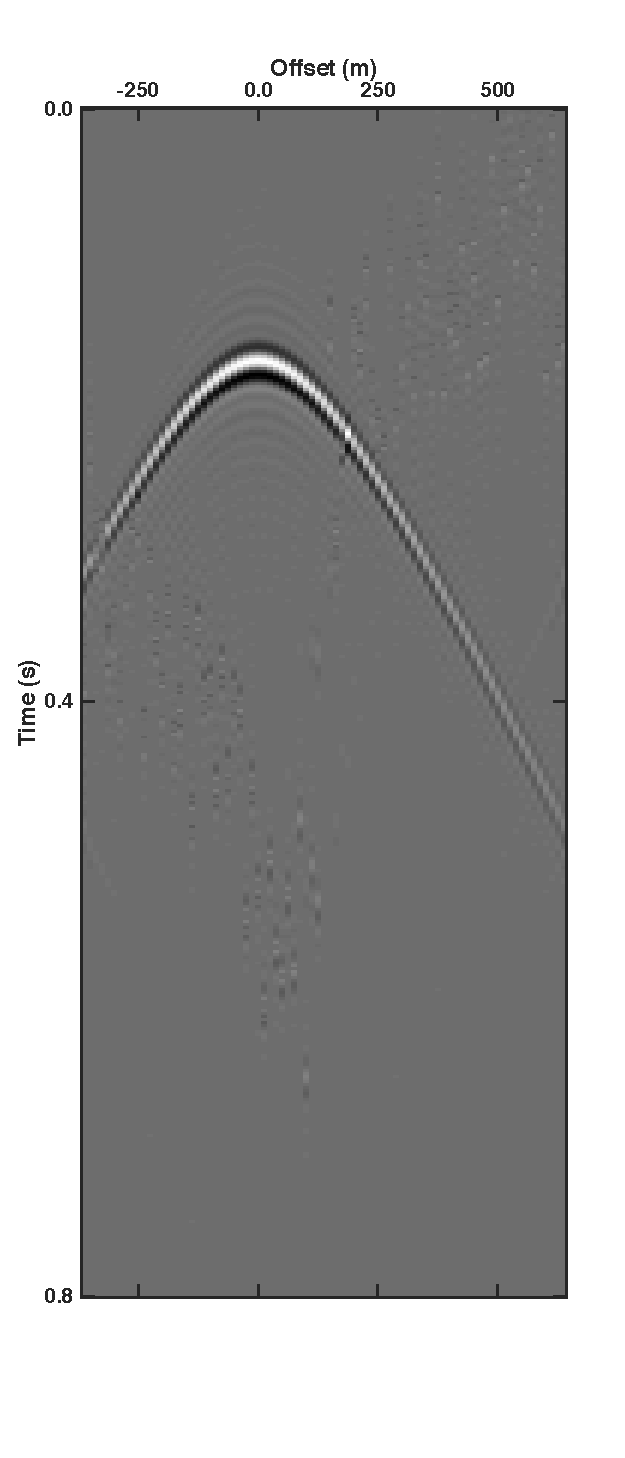
\includegraphics[width=\textwidth]{Plots/Mahdad/20iter/DeblendedCRG_rec30}	
		\caption{20 Iterations}
		\label{fig:Ch-Theory-DeblendedCRG20}
	\end{subfigure}
	%
	\begin{subfigure}[t]{0.25\textwidth}
		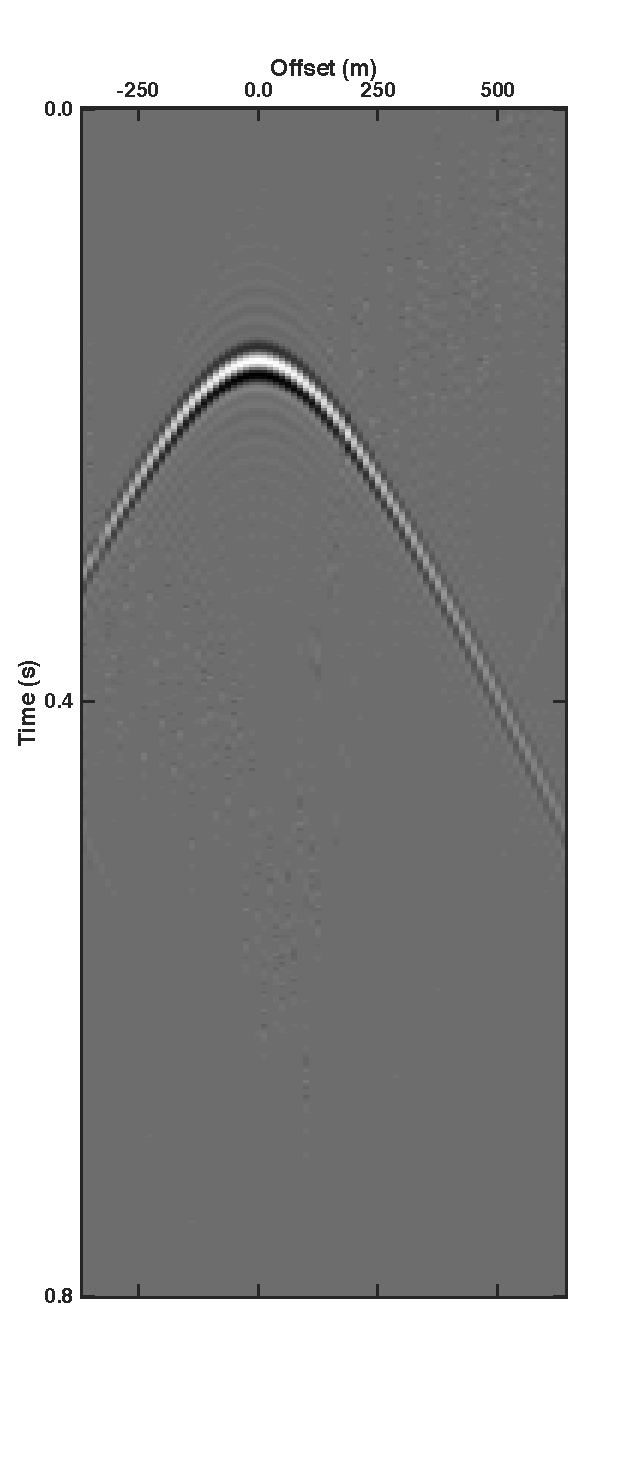
\includegraphics[width=\textwidth]{Plots/Mahdad/25iter/DeblendedCRG_rec30}	
		\caption{25 Iterations}
		\label{fig:Ch-Theory-DeblendedCRG25}
	\end{subfigure}
	\caption{Common-receiver gather of the estimated data after 1, 5, 10, 15, 20 and 25 iterations.}
	\label{fig:Ch-Theory-EstimatedData}

\end{figure}

\FloatBarrier


